\section{Analysis}

Although accuracy on some reasoning-oriented tasks is low, performance on TemporalBench does not reflect a uniform floor effect. Instead, accuracy varies systematically across task families, domains, reasoning requirements, and agent designs, revealing structured capability differences rather than metric saturation. In this section, we analyze these patterns to move beyond aggregate scores and characterize how temporal competencies emerge and fail under controlled settings.



\subsection{Analysis of Temporal Reasoning}

\begin{figure}[htbp]
\vspace{-10pt}
    \centering
 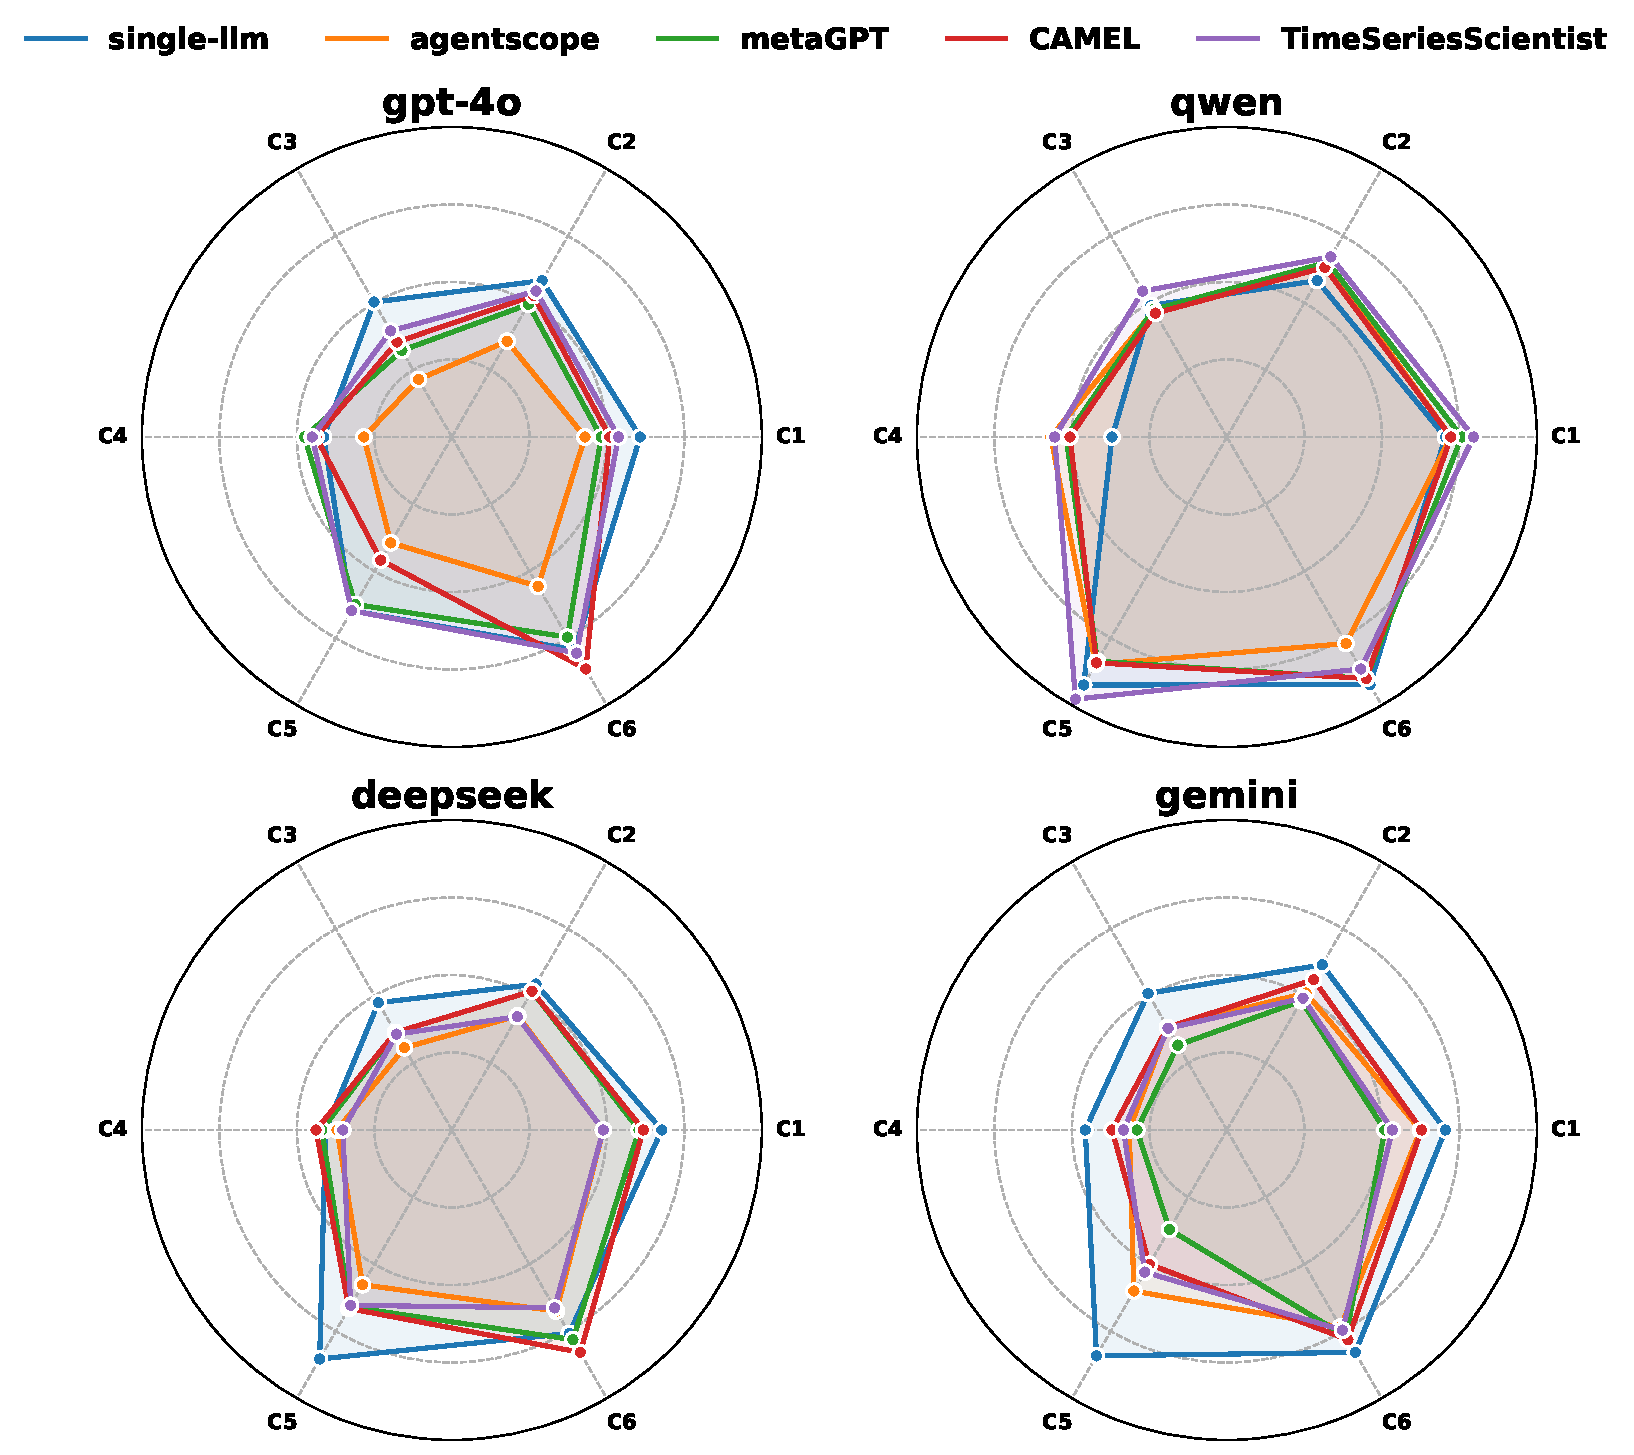
\includegraphics[width=\columnwidth]{images/radar_acc_multi.pdf}
    \caption{
Radar plots showing the performance of different agents on the six T3 reasoning dimensions (C1--C6) under different base LLMs.
Each subplot corresponds to a base model, and each curve represents an agent.
}

    \label{fig:t3_radar}
    \vspace{-30pt}
\end{figure}
To further understand agent reasoning behavior beyond aggregate accuracy, we analyze performance on T3 tasks by decomposing them into six reasoning capabilities (C1–C6). Figure~\ref{fig:t3_radar} visualizes accuracy across all agents and four backbone models. Rather than exhibiting uniform improvements, agents show highly uneven capability profiles.

Across all backbone models, C6 (interaction understanding) and C5 (structural pattern recognition) consistently achieve higher accuracy than other capabilities. These tasks primarily rely on recognizing co-occurring conditions, peak patterns, or regime-level changes, which are more amenable to surface-level pattern matching and statistical cues. In contrast, C2 (slicing-based comparison) and C3 (difference judgment) remain challenging for most agents, indicating persistent difficulty in reliably comparing temporal segments or quantifying relative changes.

Comparing agent types, general-purpose agents such as MetaGPT and CAMEL exhibit modest gains over the single-LLM baseline on higher-level reasoning dimensions (e.g., C5 and C6), but often underperform on lower-level analytical capabilities such as C1 (alignment) and C4 (lag detection). This suggests that language-driven orchestration can help with abstract interpretation but does not reliably improve fine-grained temporal analysis.

The time-series–specific agent shows a distinct but limited advantage profile. While its performance does not dominate across all six capabilities, it demonstrates more balanced behavior on C1 and C4, which require explicit temporal alignment and response-window reasoning. This pattern is consistent with its design emphasis on structured time-series processing. However, it does not substantially improve performance on higher-level comparative or interaction-based reasoning, reinforcing that specialized temporal modeling alone is insufficient for complex reasoning tasks.

Overall, the C1–C6 analysis reveals that current agents possess fragmented reasoning capabilities rather than unified temporal intelligence. Strengths in interaction and structure recognition coexist with weaknesses in comparative and causal reasoning, highlighting the need for benchmarks that disentangle reasoning dimensions and for agent designs that explicitly address these gaps.

\begin{insightbox}
\textbf{Insight.}
Temporal reasoning in current agents appears non-uniform, with structural and interaction reasoning (C5–C6) more accessible than comparative and distributional reasoning (C2–C3), suggesting that T3 failures are linked to specific reasoning gaps rather than data scarcity or model size.
\end{insightbox}



\subsection{The Role of Temporal Representations in Agent Reasoning}

To further diagnose the limitations of general-purpose agents on temporal tasks, we design a lightweight feature extraction and visualization module and integrate it into a representative general agent, AgentScope with \texttt{gpt-4o} as the backbone. In contrast to time-series–specific agents, general agents typically ingest temporal data by directly serializing numerical values into long textual prompts, without any dedicated mechanism to expose temporal structure. Such raw serialization obscures relationships among values, making it difficult for LLMs to reason about trends, volatility changes, or structural shifts over time.

\paragraph{Module Design}
The proposed module augments the raw time-series input with two complementary representations. First, we extract a compact set of structured numerical features that summarize global statistics and multi-scale temporal dynamics. This includes a reduced subset of interpretable catch22 features~\cite{lubba2019catch22} capturing distributional properties, complexity, and outliers, as well as multi-scale structural features such as short-, mid-, and long-term slopes, recent volatility, and shift indicators. All features are explicitly described in natural language within the prompt to ensure interpretability. Second, we generate a visualization of the time series, which is provided as an additional modality. The visualization exposes relative changes, peaks, and structural patterns that are difficult to infer from raw numeric tokens alone.

\paragraph{Impact on Temporal Understanding}
We evaluate the effect of this module on AgentScope by comparing its performance under different input representations.
Table~\ref{tab:feature_visual_ablation} reports results under raw time-series inputs, feature-based augmentation, visualization-based augmentation, and their combination.
Overall, the impact of enhanced representations is heterogeneous across domains and task families rather than uniformly positive.

In domains with clearer temporal structure and stronger signal-to-noise ratios, such as \emph{Causal Chambers}, enhanced representations lead to consistent improvements on multi-choice prediction and reasoning tasks, particularly for future-related judgments (T2) and event-aware prediction (T4).
In contrast, for more complex and noisy real-world domains such as \emph{FreshRetailNet} and \emph{PSML}, the gains are limited and sometimes mixed: while historical understanding (T1) often benefits from explicit structural cues, performance on reasoning-intensive tasks (T3) and future multi-choice prediction (T2) does not consistently improve and may even degrade in certain settings.

These results suggest that explicitly exposing temporal structure through features and visualizations can alleviate some failure modes of general agents, especially in structured domains.
However, representation-level augmentation alone is insufficient to resolve the broader challenges of temporal reasoning and decision-making in complex real-world time-series.
Importantly, all observed effects are obtained without additional training, task-specific tuning, or changes to the agent workflow, indicating that representation quality is a meaningful but partial factor in agent performance on time-series tasks.


\begin{insightbox}
\textbf{Insight.}
Explicit temporal representations can partially alleviate reasoning failures, but their effectiveness is domain- and task-dependent. Improvements emerge primarily in settings with clearer temporal structure, suggesting that representation quality is a necessary but insufficient condition for robust contextual and event-aware temporal reasoning.
\end{insightbox}



\begin{table}[htbp]
\vspace{-10pt}
\centering
\footnotesize
\setlength{\tabcolsep}{2.6pt}
\renewcommand{\arraystretch}{1}

% a short vertical bar (per-row), so it won't connect to top/bottom rules
\newcommand{\rowvbar}{\raisebox{-0.55ex}{\rule{0.45pt}{2.6ex}}}

\begin{tabular}{lcccc c cccc}
\toprule
& \multicolumn{4}{c}{\textbf{FreshRetailNet}} & & \multicolumn{4}{c}{\textbf{PSML}} \\
\cmidrule(lr){2-5}\cmidrule(lr){7-10}
\textbf{} & \textbf{T1} & \textbf{T2} & \textbf{T3} & \textbf{T4} & \rowvbar
& \textbf{T1} & \textbf{T2} & \textbf{T3} & \textbf{T4} \\
\midrule
\textbf{Raw}      & 62.50\% & 12.12\% & \textbf{13.64\%} & 18.94\% & \rowvbar & 66.00\% & 24.67\% & \textbf{27.20\%} & 35.33\% \\
\textbf{Feat.}       & 64.20\% & \textbf{16.67\%} & \textbf{13.64\%} & 18.94\% & \rowvbar & 63.00\% & \textbf{30.61\%} & 26.80\% & 29.33\% \\
\textbf{Vis.}   & 63.64\% & 9.09\%  & 10.80\% & \textbf{20.45\%} & \rowvbar & \textbf{67.50\%} & 26.67\% & 22.00\% & 34.67\% \\
 \textbf{Both}   & \textbf{69.32\%} & 5.30\% & 10.80\% & 15.15\% & \rowvbar & 65.00\% & 21.77\% & 21.20\% & \textbf{40.67\%} \\
\midrule
& \multicolumn{4}{c}{\textbf{MIMIC}} & & \multicolumn{4}{c}{\textbf{Causal Chambers}} \\
\cmidrule(lr){2-5}\cmidrule(lr){7-10}
\textbf{} & \textbf{T1} & \textbf{T2} & \textbf{T3} & \textbf{T4} & \rowvbar
& \textbf{T1} & \textbf{T2} & \textbf{T3} & \textbf{T4} \\
\midrule
\textbf{Raw}      & \textbf{44.68\%} & 21.28\% & 23.95\% & 22.70\% & \rowvbar & 12.00\% & 46.00\% & \textbf{44.00\%} & 32.00\% \\
\textbf{Feat.}        & 43.62\% & \textbf{25.53\%} & 24.46\% & 21.99\% & \rowvbar & \textbf{13.33\%} & 36.67\% & 42.40\% & 30.00\% \\
 \textbf{Vis.}   & \textbf{44.68\%} & 22.70\% & \textbf{26.02\%} & 24.11\% & \rowvbar & \textbf{13.33\%} & 41.33\% & 40.00\% & 36.00\% \\
 \textbf{Both}   & 44.15\% & 24.11\% & 25.43\% & \textbf{24.82\%} & \rowvbar & 10.67\% & \textbf{52.67\%} & 42.00\% & \textbf{38.67\%} \\
\bottomrule
\end{tabular}


\caption{Multi-choice accuracy (ACC) of AgentScope with \texttt{gpt-4o} under different temporal representations.
\textit{Feat.} denotes feature-based augmentation, \textit{Vis.} denotes visualization-based augmentation, and \textit{Both} indicates the combination of feature and visualization augmentations.
Bold indicates the best performance within each dataset and task column.}
\label{tab:feature_visual_ablation}

\end{table}
\vspace{-20pt}








